\section{Correctness of Parallel String Matching}\label{sec:stringmatching}

In \S~\ref{sec:parallelization} we showed that any monoid morphism
whose domain is chunkable can be parallelized. We now apply that
result to parallelize string matching. We start by observing that
strings are a chunkable monoid. %\NV add monoid methods
We then turn string matching for a
given target into a monoid morphism from a string to a suitable
monoid, @SM target@, defined in
\S~\ref{subsec:stringmatcher}. 
Finally, in \S~\ref{subsec:parallel-string-matching}, we parallelize string matching
by a simple use of the
parallel morphism function of \S~\ref{subsec:both-levels}. 

\ignore{
  In this section we apply the Correctness of Parallelization Theorem~\ref{theorem:two-level}
to a string matching function @toSM@
that is a morphism between strings and the indices where a target string appears,
to get correctness of parallelization of @toSM@.

We define @toSM :: RString -> SM target@
from a Refined String data type @RString@
to a dependently typed string maching data type @SM target@
where @target@ represents the substring to be matched.
%
To apply Theorem~\ref{theorem:two-level} on @toSM@ we need to discharge three proof obligations.
%
\begin{itemize}
\item @RString@ is a chunkable monoid (\S~\ref{subsec:refinedstrings}),
\item @SM target@ is a monoid (\S~\ref{subsec:stringmatcher}), and
\item @toSM@ is a morphism between @RString@ and @SM target@ (\S~\ref{subsec:smmorphism}).
\end{itemize}
%
With these proof obligations discharged we conclude (\S~\ref{subsec:parallel-string-matching})
correctness of parallel string matching.
}

\subsection{Refined Strings are Chunkable Monoids}\label{subsec:refinedstrings}
We define a new type @RString@, which is a chunkable monoid, to be the
domain of our string matching function. Our type simply wraps
Haskell's existing @ByteString@.
\begin{code}
data RString = RS BS.ByteString
\end{code}
Similarly, we wrap the existing @ByteString@ functions we will need to
show @RString@ is a chunkable monoid.
\begin{code}
stringMempty = RS (BS.empty)
(RS x) stringMappend (RS y)= S (x `BS.append` y)

lenStr    (RS x) = BS.length x
takeStr i (RS x) = RS (BS.take i x)
dropStr i (RS x) = RS (BS.take i x)
\end{code}
Although it is possible to explicitly prove that @ByteString@
implements a chunkable monoid~\cite{realworldliquid14}, it is time
consuming and orthogonal to our purpose. Instead, we
just \textit{assume} the chunkable monoid properties of @RString@--
thus demonstrating that refinement reflection is capable of doing
gradual verification.


\ignore{
We follow the easy route, defining the @RString@ data type to be a wrapper of the
optimized @ByteString@ and

%
This allows our implementation to \textit{use the optimized library
functions} of @ByteString@; additionally, it shows that refinement
reflection can be used for \textit{gradual verification} where
verified code uses untrusted components that are explicitely assumed
to satisfy required properties.
%
Proving that @ByteString@ implements a chunkable monoid is feasible,
as evidenced by the current verification of Bytestring functions~\cite{realworldliquid14},
but it is time consuming and orthogonal to the string matching proof.
%
%% NV I need to automate this in LiquidHaskell!

We need to use the above operators to specify the chunkable monoid
laws, but we cannot reflect the operators in the logic, as the
ByteString functions do not exist in the logic.  We ``manually
reflect'' each of the above functions in the logic, by 1. defining a
logical uninterpreted function for each of them that assumed to be
equal to the Haskell functions and 2. use the logical functions to
specify the chunkable monoid laws.
}

For instance, we define a logical uninterpreted function
@stringMappend@ and relate it to the Haskell @stringMappend@ function
via an assumed (unchecked) type.
%
\begin{code}
assume (stringMappend)
  :: x:RString -> y:RString -> {v:RString | v = x stringMappend y}
\end{code}
%
Then, we use the uninterpreted function @stringMappend@ in the logic
to assume monoid laws, like associativity.
%
\begin{code}
assume assocStr :: x:RString -> y:RString -> z:RString
                 -> { x <+> (y <+> z) = (x <+> y) <+> z }
assocStr _ _     = trivial
\end{code}
%
Haskell applications of @stringMappend@ are interpreted in the logic
via the logical @stringMappend@ that satisfies associativity via theorem @assocStr@.

Similarly for the chunkable methods, we define the uninterpreted functions
@takeStr@, @dropStr@ and @lenStr@ in the logic,
and use them to strengthen the result types of the respective functions.
%
\ignore{
For example the type of @takeStr@ includes both the length specifications
from chunkable monoid and the uninterpreted function equality @v = takStr i x@.
\begin{code}
assume takeStr
  :: i:Nat -> x:{RString | i <= lenStr x}
  ->  {v:RString | lenStr v = i && v = takeStr i x }
\end{code}
We use the uninterpreted function @takeStr@ and @dropStr@ to
specify and \textit{assume} the @take@-@drop@ property of chunkable monoids.
\begin{code}
assume takeDropPropStr
 :: i:Nat -> x:RString -> {x = takeStr i x <+> dropStr i x}
takeDropPropStr _ _ = trivial
\end{code}
%
} With the above function definitions (in both Haskell and logic) and
assumed type specifications, Liquid Haskell will check (or rather
assume) that the specifications of chunkable monoid, as defined in the
Definitions~\ref{definition:monoid} and~\ref{definition:chunkable},
are satisfied.
%
We conclude with the assumption (rather that theorem)
that @RString@ is a chunkable monoid.
\begin{assumption}[RString is a Chunkable Monoid]\label{assumption:rstring}
(@RString@, @stringMempty@, @stringMappend@)
combined with the methods
@lenStr@, @takeStr@, @dropStr@ and @takeDropPropStr@
is a chunkable monoid.
\end{assumption}


\subsection{String Matching Monoid}\label{subsec:stringmatcher}
String matching is determining all the indices in a source string
where a given target string begins; for example, for source string
\texttt{ababab} and target \texttt{aba} the results of string
matching would be \texttt{[0, 2]}. 

We now define a suitable monoid, @SM target@, for the codomain of
a string matching function, where @target@ is the string being looked
for.
%
Additionally, we will define a function @toSM :: RString -> SM target@
which does the string matching and is indeed a monoid morphism from
@RString@ to @SM target@ for a given @target@.

\subsubsection{String Matching Monoid}

We define the data type
@SM target@ to contain a refined string field @input@ and
a list of all the indices in @input@ where the
@target@ appears.
%
\begin{code}
  data SM (target :: Symbol) where
    SM :: input:RString
       -> indices:[GoodIndex input target]
       -> SM target
\end{code}
%
We use the string type literal~\footnote{\texttt{Symbol} is a kind and
target is effectively a singleton type.} to parameterize the monoid
over the target being matched. This encoding allows the type checker
to statically ensure that only searches for the same target can be
merged together.  The input field is a refined string, and the indices
field is a list of good indices.  For simplicity we present lists as
Haskell's built-in lists, but our implementation uses the reflected
list type, @L@, defined in \S~\ref{sec:haskell-proofs}.

A @GoodIndex input target@ is a refined type alias for a natural
number @i@ for which @target@ appears at position @i@ of @input@.  As
an example, the good indices of @"abcab"@ on @"ababcabcab"@ are
@[2,5]@.
%
\begin{code}
  type GoodIndex Input Target
    = {i:Nat | isGoodIndex Input (fromString Target) i }

  isGoodIndex :: RString -> RString -> Int -> Bool
  isGoodIndex input target i
    = (subString i (lenStr target) input  == target)
    && (i + lenStr target <= lenStr input)

  subString :: Int -> Int -> RString -> RString
  subString o l = takeStr l . dropStr o
\end{code}
%
\ignore{
\begin{code}
goodSM :: SM "abcab"
goodSM = SM "ababcabcab" [2, 5]

badSM  :: SM "abcab"
badSM  = SM "ababcabcab" [0, 7]
\end{code}
\ignore{
\NV{Liquid Haskell actually will reject both the above, as the lenStr and subString functions are uninterpreted}
}
}

\subsubsection{Monoid Methods for String Matching}~\label{subsec:monoid:methods}
Next, we define the mappend and identity elements for string matching.

The \textit{identity element} @mempty@ of @SM t@, for each target @t@, is
defined to contain the identity @RString@ (@stringMempty@) and the
identity @List@ (@listMempty@).
\begin{code}
  mempty:: forall (t :: Symbol). SM t
  mempty = SM stringMempty listMempty
\end{code}
%

\ignore{
The associative operator, @(mappend)@,
appends the two input strings.
The appended indices, as depicted in Figure~\ref{fig:mappend:indices},
are the concatenations of three list indices:
\begin{enumerate}
\item The indices @xis@ of the first input, casted to good indices in the new structure,
\item the new indices @xyis@ created when concatenating the two strings, and
\item the indices @yis@ of the second input, shifted right @lenStr y@ units.
\end{enumerate}
%
}

\begin{figure}[t]
\centering
\captionsetup{justification=centering}
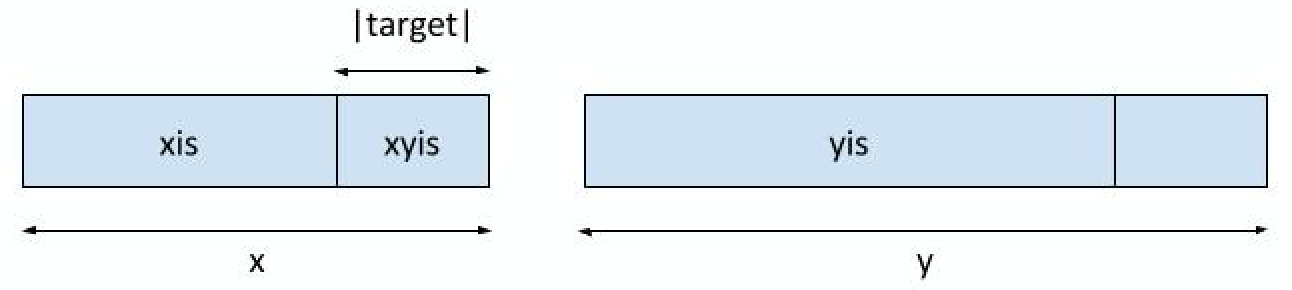
\includegraphics[scale=0.5]{text/stringmatcher/makeIndices}
\caption{Mappend indices of String Matcher.}
\label{fig:mappend:indices}
\end{figure}
%
The Haskell definition of @<>@, the monoid operation for @SM t@, is as follows.
\begin{code}
  (mappend)::forall (t::Symbol). KnownSymbol t => SM t -> SM t -> SM t
  (SM x xis) mappend (SM y yis)
    = SM (x stringMappend y) (xis' listMappend xyis listMappend yis')
    where
      tg   = fromString (symbolVal (Proxy :: Proxy t))
      xis' = map (castGoodIndexLeft tg x y) xis
      xyis = makeNewIndices x y tg
      yis' = map (shiftStringRight tg x y) yis
\end{code}
Note again that capturing target as a type parameter is critical,
otherwise there is no way for the Haskell's type system to specify
that both arguments of @(mappend)@ are string matchers on the same target.

The action of @(<>)@ on the two @input@ fields is straightforward;
however, the action on the two @indices@ is complicated by the need to
shift indices and the possibility of new matches arising from the
concatenation of the two @input@
fields. Figure~\ref{fig:mappend:indices} illustrates the three pieces
of the new @indices@ field which we now explain in more detail.

\mypara{1. Casting Good Indices}
If @xis@ is a list of good indices for the string @x@ and the target
@tg@, then @xis@ is also a list of good indices for the string
@x stringMappend y@ and the target @tg@, for each @y@.
%
To prove this property we need to invoke the property
@subStrAppendRight@ on Refined Strings that establishes
substring preservation on string right appending.
%
\begin{code}
  assume subStrAppendRight
      :: sl:RString -> sr:RString -> j:Int
      -> i:{Int | i + j <= lenStr sl }
      -> {subString sl i j = subString (sl stringMappend sr) i j}
\end{code}
%
The specification of @subStrAppendRight@ ensures that for each
string @sl@ and @sr@ and each integer @i@ and @j@ whose sum is within @sl@,
the substring from @i@ with length @j@ is identical in @sl@ and in @(sl stringMappend sr)@.
%
The function @castGoodIndexLeft@ applies the above property to an index @i@
to cast it from a good index on @sl@ to a good index on @(sl stringMappend sr)@
%
\begin{code}
  castGoodIndexLeft
    :: tg:RString -> sl:RString -> sr:RString
    -> i:GoodIndex sl tg
    -> {v:GoodIndex (sl stringMappend sr) target | v = i}

  castGoodIndexLeft tg sl sr i
    = cast (subStrAppendRight sl sr (lenStr tg) i) i
\end{code}
%
Where @cast p x@ returns @x@, after enforcing the properties of @p@ in the logic
\begin{code}
  cast :: b -> x:a -> {v:a | v = x}
  cast _ x = x
\end{code}
%
Moreover, in the logic, each expression @cast p x@
is reflected as @x@,
thus allowing random (\ie non-reflected) Haskell expressions to appear in @p@.

\mypara{2. Creation of new indices}
The concatenation of two input strings @sl@ and @sr@
may create new good indices.
%
For instance, concatenation of
@"ababcab"@ with @"cab"@
leads to a new occurence of @"abcab"@ at index @5@ which
does not occur in either of the two input strings.
%
These new good indices can appear only at the last @lenStr tg@ positions
of the left input @sl@.
%
@makeNewIndices sl sr tg@ detects all such good new indices.
%
\begin{code}
  makeNewIndices
    :: sl:RString -> sr:RString -> tg:RString
    -> [GoodIndex {sl stringMappend sr} tg]
    
  makeNewIndices sl sr tg
    | lenStr tg < 2 = []
    | otherwise     = makeIndices (sl stringMappend sr) tg lo hi
    where
      lo = maxInt (lenStr sl - (lenStr tg - 1)) 0
      hi = lenStr sl - 1
\end{code}
If the length of the @tg@ is less than 2, then no new good indices are created.
%
Otherwise,
the call on @makeIndices@ returns all the good indices of the input
@sl stringMappend sr@ for target @tg@
in the range from @maxInt (lenStr sl-(lenStr tg-1)) 0@ to  @lenStr sl-1@.
%

Generally, @makeIndices s tg lo hi@ returns the good indices
of the input string @s@ for target @tg@ in the range from @lo@ to @hi@.
%
\begin{code}
  makeIndices :: s:RString -> tg:RString -> lo:Nat
              -> hi:Int -> [GoodIndex s tg]
    
  makeIndices s tg lo hi  
    | hi < lo             = []
    | isGoodIndex s tg lo = lo:rest
    | otherwise           = rest
    where
      rest = makeIndices s tg (lo + 1) hi
\end{code}
%Note the similarity to the functional specification of string matching
%at the beginning of this section.

It is important to note that
@makeNewIndices@ does not scan all the input,
instead only searching at most @lenStr tg@ positions for new good indices.
%
Thus, the time complexity to create the new indices is linear
on the size of the target but independent of the size of the input.

\mypara{3. Shift Good Indices}
If @yis@ is a list of good indices on the string @y@ with target @tg@,
then we need to shift each element of @yis@ right @lenStr x@ units to
get a list of good indices for the string @x stringMappend y@.

%
To prove this property we need to invoke the property
@subStrAppendLeft@ on Refined Strings that establishes
substring shifting on string left appending.
%
\begin{code}
  assume subStrAppendLeft
    :: sl:RString -> sr:RString
    -> j:Int -> i:Int
    -> {subStr sr i j = subStr (sl stringMappend sr) (lenStr sl+i) j}
\end{code}
%
The specification of @subStrAppendLeft@ ensures that for each
string @sl@ and @sr@ and each integers @i@ and @j@,
the substring from @i@ with length @j@ on @sr@
is equal to the substring from @lenStr sl + i@
with length @j@ on @(sl stringMappend sr)@.
%
The function @shiftStringRight@ both shifts the input index @i@ by @lenStr sl@
and applies the @subStrAppendLeft@ property to it,
casting @i@ from a good index on @sr@ to a good index on @(sl stringMappend sr)@

Thus, @shiftStringRight@ both appropriately shifts the index
and casts the shifted index using the above theorem:
\begin{code}
  shiftStringRight
    :: tg:RString -> sl:RString -> sr:RString
    -> i:GoodIndex sr tg
    -> {v:(GoodIndex (sl stringMappend sr) tg) | v = i + lenStr sl}
    
  shiftStringRight tg sl sr i
    = subStrAppendLeft sl sr (lenStr tg) i `cast` i + lenStr sl
\end{code}

\subsubsection{String Matching is a Monoid}
Next we prove that the monoid methods @mempty@ and @(mappend)@ satisfy
the monoid laws.
%
\begin{theorem}[SM is a Monoid]\label{theorem:stringmatchers}
(@SM t@, @mempty@, @mappend@)
is a monoid.
\end{theorem}
%
\begin{proof}
According to the Monoid Definition~\ref{definition:monoid},
we prove that string matching is a monoid,
by providing safe implementations for the monoid law functions.
%
First, we prove \textit{left identity}.
\begin{code}
  idLeft :: x:SM t -> {mempty mappend x = xs}
  
  idLeft (SM i is)
    =   (mempty :: SM t) mappend (SM i is)
    =. (SM stringMempty listMempty) mappend (SM i is)
    =. SM (stringMempty <+> i) (is1 ++ isNew ++ is2)
       ? idLeftStr i
    =. SM i ([] ++ [] ++ is)
       ? (mapShiftZero tg i is && newIsNullRight i tg)
    =. SM i is
       ? idLeftList is
    ** QED
    where
      tg    = fromString (symbolVal (Proxy :: Proxy t))
      is1   = map (castGoodIndexRight tg i stringMempty) []
      isNew = makeNewIndices stringMempty i tg
      is2   = map (shiftStringRight tg stringMempty i) is
\end{code}

The proof proceeds by rewriting, using left identity of the monoid strings and lists,
and two more lemmata.
\begin{itemize}
\item Identity of shifting by an empty string.
\begin{code}
  mapShiftZero :: tg:RString -> i:RString
    -> is:[GoodIndex i target]
    -> {map (shiftStringRight tg stringMempty i) is = is}
\end{code}
The lemma is proven by induction on @is@ and
the assumption that empty strings have length 0.
\item No new indices are created.
\begin{code}
  newIsNullLeft :: s:RString -> t:RString 
                -> {makeNewIndices stringMempty s t = []}
\end{code}
The proof relies on the fact that @makeIndices@
is called on the empty range from @0@ to @-1@
and returns @[]@.
\end{itemize}

Next, we prove \textit{right identity}.
\begin{code}
  idRight :: x:SM t -> {x mappend mempty = x}
  
  idRight (SM i is)
    =  (SM i is) mappend (mempty :: SM t)
    =. (SM i is) mappend (SM stringMempty listMempty)
    =. SM (i stringMappend stringMempty) (is1 listMappend isNew listMappend is2)
       ? idRightStr i
    =. SM i (is listMappend N listMappend N)
       ? (mapCastId tg i stringMempty is && newIsNullLeft i tg)
    =. SM i is
       ? idRightList is
    **  QED
    where
      tg    = fromString (symbolVal (Proxy :: Proxy t))
      is1   = map (castGoodIndexRight tg i stringMempty) is
      isNew = makeNewIndices i stringEmp tg
      is2   = map (shiftStringRight tg i stringMempty) []
\end{code}
The proof proceeds by rewriting,
using right identity on strings and lists and two more lemmata.
\begin{itemize}
\item Identity of casting is proven
\begin{code}
  mapCastId 
    :: tg:RString -> x:RString -> y:RString
    -> is:[GoodIndex x tg] ->
    -> {map (castGoodIndexRight tg x y) is = is}
\end{code}
We prove identity of casts by induction on @is@ and
identity of casting on a single index.
\item No new indices are created.
\begin{code}
  newIsNullLeft 
    :: s:RString -> t:RString
    -> {makeNewIndices s stringMempty t = listMempty}
\end{code}
The proof proceeds by case splitting
on the relative length of @s@ and @t@.
At each case we prove by induction that all
the potential new indices would be out of bounds and thus
no new good indices would be created.
\end{itemize}

- Finally we prove \textit{associativity}.
For space, we only provide a proof sketch.
The whole proof is available online~\cite{implementation}.
%
Our goal is to show equality of the left and right associative string matchers.
%
\begin{code}
  assoc :: x:SM t -> y:SM t -> z:SM t
        -> {x mappend (y mappend z) = (x mappend y) mappend z}
\end{code}
To prove equality of the two string matchers we show
that the input and indices fields are respectively equal.
%
Equality of the input fields follows by associativity of RStrings.
%
Equality of the index list proceeds in three steps.
%
\begin{enumerate}
\item Using list associativity and distribution of index shifting,
we group the indices in the five lists shown in
Figure~\ref{fig:mappend:assoc}: the indices of the input @x@, the new
indices from mappending @x@ to @y@, the indices of the input @y@, the
new indices from mappending @x@ to @y@, and the indices of the input
@z@.
\item The representation of each group depends on the order of appending.
For example, if @zis1@ (resp. @zis2@) is the group @zis@ when
right (resp. left) mappend happened first, then we have
\begin{code}
  zis1 = map (shiftStringRight tg xi (yi stringMappend zi))
             (map (shiftStringRight tg yi zi) zis)

  zis2 = map (shiftStringRight tg (xi stringMappend yi) zi) zis
\end{code}
That is, in right first, the indices of @z@ are first shifted
by the length of @yi@ and then by the length of @xi@,
while in the left first case, the indices of @z@ are shifted by the
length of @xi stringMappend yi@.
In this second step of the proof we prove, using lemmata,
the equivalence of the different group representations.
%
The most interesting lemma we use is called @assocNewIndices@ and proves
equivalence of all the three middle groups together
by case analysis on the relative lengths of the target @tg@ and the middle string @yi@.
\item After proving equivalence of representations,
we again use list associativity and distribution of casts to wrap the
index groups back in string matchers.
\end{enumerate}
\begin{figure}
\centering
\captionsetup{justification=centering}
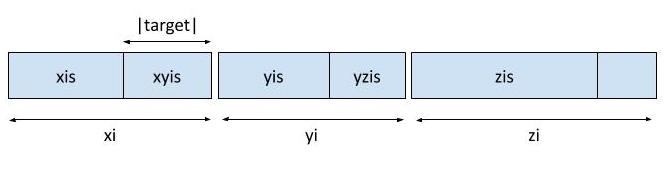
\includegraphics[scale=0.5]{text/stringmatcher/AssociativeIndices}
\caption{Associativity of String Matching.}
\label{fig:mappend:assoc}
\end{figure}
We now sketch the three proof steps, while the whole proof
is available online~\cite{implementation}.
\begin{code}
  assoc x@(SM xi xis) y@(SM yi yis) z@(SM zi zis)
    -- Step 1: unwrapping the indices
    =   x <> (y <> z)
    =. (SM xi xis) <> ((SM yi yis) <> (SM zi zis))
                         ...
    -- via list associativity and distribution of shifts
    =. SM i (xis1 ++ ((xyis1 ++ yis1 ++ yzis1) ++ zis1))
    -- Step 2: Equivalence of representations
    =. SM i (xis2 ++ ((xyis1 ++ yis1 ++ yzis1) ++ zis1))
       ? castConcat tg xi yi zi xis
    =. SM i (xis2 ++ ((xyis1 ++ yis1 ++ yzis1) ++ zis2))
       ? mapLenFusion tg xi yi zi zis
    =. SM i (xis2 ++ ((xyis2 ++ yis2 ++ yzis2) ++ zis2))
       ? assocNewIndices y tg xi yi zi yis
    -- Step 3: Wrapping the indices
                         ...
    -- via list associativity and distribution of casts
    =. (SM xi xis <> SM yi yis) <> SM zi zis
    =. (x <> y) <> z
    ** QED
    where
      i     = xi stringMappend (yi stringMappend zi)

      yzis1 = map (shiftStringRight tg xi (yi <+> zi)) yzis
      yzis2 = makeNewIndices (xi <+> yi) zi tg
      yzis  = makeNewIndices yi zi tg
      ...
\end{code}
\cqed\end{proof}


\subsection{String Matching Monoid Morphism}\label{subsec:smmorphism}
Next, we define the function @toSM :: RString -> SM target@ which does
the actual string matching computation for a set
target~\footnote{\texttt{toSM} assumes the target is clear from the
  calling context; it is also possible to write a wrapper function
  taking an explicit target which gets existentially reflected into
  the type.}
%
\ignore{ The function @toSM input@ creates a string matcher @SM
  target@ structure that matches the type level symbol target to the
  string value argument @input@.  }
%
\begin{code}
toSM :: forall (target :: Symbol). (KnownSymbol target)
     => RString -> SM target
toSM input = SM input (makeSMIndices input tg) where
  tg = fromString (symbolVal (Proxy :: Proxy target))

makeSMIndices
  :: x:RString -> tg:RString -> [GoodIndex x tg]
makeSMIndices x tg
  = makeIndices x tg 0 (lenStr tg - 1)
\end{code}
%
The input field of the result is the input string;
the indices field is computed by calling @makeIndices@
within the range of the @input@, that is from
@0@ to @lenStr input - 1@.
%
\begin{code}
\end{code}

We now prove that @toSM@ is a monoid morphism.
%
\begin{theorem}[$\texttt{toSM}$ is a Morphism]\label{theorem:smmorphism}
@toSM :: RString -> SM t@ is a morphism between the monoids
(@RString@, @stringMempty@, @stringMappend@) and (@SM t@, @mempty@, @mappend@).
\end{theorem}
\begin{proof}
Based on definition~\ref{definition:morphism}, proving @toSM@
is a morphism requires constructing a valid inhabitant of the type
\begin{code}
Morphism RString (SM t) toSM
  = x:RString -> y:RString
  -> {toSM stringMempty = mempty && toSM (x <+> y) = toSM x <> toSM y}
\end{code}
%
We define the function @distributestoSM :: Morphism RString (SM t) toSM@
to be the required valid inhabitant.

The core of the proof starts from
exploring the string matcher @toSM x <> toSM y@.
%
This string matcher contains three sets of indices
as illustrated in Figure~\ref{fig:mappend:indices}:
(1) @xis@ from the input @x@,
(2) @xyis@ from appending the two strings, and
(3) @yis@ from the input @y@.
%
We prove that appending these three groups of indices together gives
exactly the good indices of @x stringMappend y@, which are also the
value of the indices field in the result of
%
@toSM (x stringMappend y)@.
\begin{code}
distributestoSM x y
  =   (toSM x :: SM target) <> (toSM y :: SM target)
  ==. (SM x is1) <> (SM y is2)
  ==. SM i (xis ++ xyis ++ yis)
  ==. SM i (makeIndices i tg 0 hi1 ++ yis)
      ? (mapCastId tg x y is1 && mergeNewIndices tg x y)
  ==. SM i (makeIndices i tg 0       hi1
         ++ makeIndices i tg (hi1+1) hi)
      ? shiftIndicesRight 0 hi2 x y tg
  ==. SM i is
      ? mergeIndices i tg 0 hi1 hi
  ==. toSM (x <+> y)
  *** QED
  where
    xis  = map (castGoodIndexRight tg x y) is1
    xyis = makeNewIndices x y tg
    yis  = map (shiftStringRight   tg x y) is2
    tg   = fromString (symbolVal (Proxy::Proxy target))
    is1  = makeSMIndices x tg
    is2  = makeSMIndices y tg
    is   = makeSMIndices i tg
    i    = x <+> y
    hi1  = lenStr x - 1
    hi2  = lenStr y - 1
    hi   = lenStr i - 1
\end{code}
%
The most interesting lemma we use is
@mergeIndices x tg lo mid hi@
that states that for the input @x@ and the target @tg@
if we append the indices in the range  from @to@ to @mid@
with the indices in the range from @mid+1@ to @hi@,
we get exactly the indices in the range from @lo@ to @hi@.
%
This property is formalized in the type of the lemma.
\begin{code}
mergeIndices
 :: x:RString -> tg:RString
  -> lo:Nat -> mid:{Int | lo <= mid} -> hi:{Int | mid <= hi}
  -> {   makeIndices x tg lo hi
     =  makeIndices x tg lo mid
     ++ makeIndices x tg (mid+1) hi}
\end{code}
%
The proof proceeds by induction on @mid@ and using three more lemmata:
\begin{itemize}
\item @mergeNewIndices@ states that appending the indices @xis@ and @xyis@
is equivalent to the good indices of @x stringMappend y@ from @0@ to @lenStr x - 1@.
%
The proof case splits on the relative sizes of @tg@ and @x@
and is using @mergeIndices@ on @mid = lenStr x1 - lenStr tg@
in the case where @tg@ is smaller than @x@.
%
\item @mapCastId@ states that casting a list of indices returns the same list.
\item @shiftIndicesRight@ states that shifting right @i@ units the indices from @lo@ to @hi@
is equivalent to computing the indices from @i + lo@
to @i + hi@ on the string @x stringMappend y@, with @lenStr x = i@.
\end{itemize}
%%\begin{code}
%%mergeNewIndices
%%  :: tg:RString -> x:RString -> y:RString
%%  -> { makeSMIndices x tg
%%    ++ makeNewIndices x y tg
%%    == makeIndices (x <+> y) tg 0 (lenStr x - 1)}
%%\end{code}
%%The theorem states that appending the indices that appear in the first string @x@,
%%that is the indices @xis@ that do not and the indices @xyis@ that do involve @y@,
%%is equivalent to the indices @is@ on the input @x stringMappend y@
%%in the range from @0@ to @lenStr x -1@.
%%%
%%The proof case splits on the sizes of @tg@ and @x@.
%%%
%%If the size of the target is less than two, then @xyis@ is empty,
%%but @xis == is@, as appending @y@ to the input cannot create more indices.
%%%
%%Otherwise, if the input @x@ is smaller than the target,
%%then @xis@ is empty and @xyis@ is equal to @is@.
%%%
%%Otherwise, we set
%%and use the previous @mergeIndices@ lemma to merge @xis@ and @yis@ into @is@.
%%\item Shifting is left concatenation.
%%\begin{code}
%%shiftIndicesRight
%%  :: lo:Nat -> hi:Int
%%  -> x:RString -> y:RString
%%  -> tg:RString
%%  -> { map (shiftStringRight tg x y)
%%           (makeIndices y tg lo hi)
%%  == makeIndices (x stringMappend y) tg
%%                 (lenStr x + lo) (lenStr x + hi) }
%%
%%\end{code}
%%The lemma states that shifting indices from @lo@ to @hi@ on @y@
%%is equivalent to computing the indices from @lenStr x + lo@
%%to @lenStr x + hi@ on @x stringMappend y@,
%%and it is proved by induction on the difference @hi - lo@.
%%\end{itemize}
\qed\end{proof}


\subsection{Parallel String Matching}\label{subsec:parallel-string-matching}
We conclude this section with
the definition of a parallelized version of string matching.
%
We put all the theorems together to prove 
that the sequential and parallel versions always give the same result.
% and compare their time complexities.

We define @toSMPar@ as a parallel version of @toSM@ using machinery of section~\ref{sec:parallelization}.
\begin{code}
toSMPar :: forall (target :: Symbol). (KnownSymbol target)
        => Int -> Int -> RString -> SM target
toSMPar i j = pmconcat i . pmap toSM . chunkStr j
\end{code}
%
First, @chunkStr@ splits the input into @j@ chunks.
%
Then, @pmap@ applies @toSM@ at each chunk in parallel.
Finally, @pmconat@ concatenates the mapped chunks in parallel
using @mappend@, the monoidal operation for @SM target@.

\paragraph{Correctness.}
We prove correctness of @toSMPar@ directly from
Theorem~\ref{theorem:two-level}.
\begin{theorem}[Correctness of Parallel String Matching]\label{theorem:correctness}
For each parameter @i@ and @j@, and input @x@,
@toSMPar i j x@ is always equal to @toSM x@.
\begin{code}
correctness :: i:Int -> j:Int -> x:RString
             -> {toSM x = toSMPar i j x}
\end{code}
\end{theorem}

\begin{proof}
The proof follows by direct application of Theorem~\ref{theorem:two-level}
on the chunkable monoid (@RString@, @$\eta$@, @<+>@) (by Assumption~\ref{assumption:rstring})
and the monoid (@SM t@, @$\epsilon$@, @<>@) (by Theorem~\ref{theorem:stringmatchers}).
%
\begin{code}
correctness i j x
  =   toSMPar i j x
  ==. pmconcat i (pmap toSM (chunkStr j x))
  ==. toSM is
    ? parallelismEquivalence toSM distributestoSM x i j
  *** QED
\end{code}
%
Note that application of the theorem @parallelismEquivalence@
requires a proof that its first argument @toSM@ is a morphism.
%
By Theorem~\ref{theorem:monoid:distribution},
the required proof is provided as the function @distributestoSM@.
\qed\end{proof}

\ignore{

\paragraph{Time Complexity.}
Counting only string comparisons as the expensive operations,
the sequential string matcher on input @x@ runs in time
linear to @n = lenStr x@. Thus $T_\texttt{toSM}(n) = O(n)$.

We get time complexity of @toSMPar@ by the time complexity of
two-level parallel algorithms equation~\ref{eq:complexity},
with the time of string matching mappend being linear on the length
of the target @t = lenStr tg@, or
$T_\mappend(\texttt{SM})= O(t)$.
%
$$
T_\texttt{toSMPar} (n, t, i, j) =
O((i-1)(\frac{\log n - \log j}{\log i}) t  + \frac{n}{j})
$$
%
The above analysis refers to a model with infinite processor and no caching.
To compare the algorithms in practice,
we matched the target "the"
in  Oscar Wilde's "The Picture of Dorian Gray", a text of @n = 431372@ characters
using a two processor Intel Core i5.
%
The sequential algorithm detected 4590 indices in 40 ms.
%
We experimented with different parallization factors @i@ and chunk sizes @j / n@
and observed up to $50\%$ speedups of the parallel algorithm for parallelization factor
@4@ and @8@ chunks.
%
As a different experiment, we matched the input against its size @t = 400@ prefix,
a size comparable to the input size @n@.
%
For bigger targets,
mappend gets slower, as it has complexity linear to the size of target.
%
We observed $20\%$ speedups for @t=400@ target but also $30\%$ slow downs for various sizes of @i@ and @j@.
%
In all cases the indices returned by the sequential and the parallel algorithms were the same.
}

